\documentclass[conference]{IEEEtran}
\usepackage{amsmath,amssymb,amsfonts}
\usepackage{graphicx}
\usepackage{textcomp}
\usepackage{xcolor}
\usepackage{booktabs}
\usepackage{hyperref}
\usepackage{subcaption}
\usepackage{algorithm}
\usepackage{algorithmic}
\usepackage{listings}

\lstset{
  basicstyle=\ttfamily\small,
  breaklines=true,
  frame=single,
  xleftmargin=1em,
  xrightmargin=1em
}

\begin{document}

\title{Deception Benchmark: A Stress-Test Benchmark for Trusted Vulnerability Detection with Honeypot Anti-Overfitting}

\author{
\IEEEauthorblockN{Anshumali Shrivastava\IEEEauthorrefmark{1}\IEEEauthorrefmark{2}\IEEEauthorrefmark{3}, Neha Rungta\IEEEauthorrefmark{1}, Alexander Greaves-Tunnell\IEEEauthorrefmark{1}}
\IEEEauthorblockA{\IEEEauthorrefmark{1}Amazon Web Services \quad \IEEEauthorrefmark{2}Rice University \quad \IEEEauthorrefmark{3}Corresponding author: anshumsh@amazon.com}
}

\maketitle

\begin{abstract}
AI-powered security tools achieve near-perfect vulnerability recall but generate false positive rates of 41--99\% on code that security engineers routinely classify correctly. This is not merely a production inconvenience: it reveals that models detect vulnerability patterns without genuinely understanding code. You cannot compensate for this with a harness; as attacks self-improve, the attack surface will outrun any static verification layer. Yet no existing benchmark measures this: current evaluations test whether models can \emph{detect} known vulnerabilities, not whether they can tell real threats from safe code that merely looks suspicious.

We introduce Deception Benchmark, a 14,822-sample benchmark spanning 16 programming languages and 70+ CWE categories, specifically designed to stress-test discrimination capability. Safe samples exhibit genuine vulnerability patterns with subtle mitigations that break the exploit chain. We evaluate 12 models from 5 providers under two prompting strategies and find that \textbf{no model achieves both FPR $<$ 10\% and FNR $<$ 10\% simultaneously}, a very generous threshold to be interesting for production use.

We additionally introduce \emph{Honeypot Benchmarking}, a novel anti-overfitting methodology that embeds deliberately ambiguous samples to structurally resist benchmark gaming. We provide a game-theoretic argument for its optimality and discuss its applicability to ML benchmarking broadly.
\end{abstract}

\begin{IEEEkeywords}
Security benchmarks, vulnerability detection, false positives, LLM evaluation, benchmark integrity
\end{IEEEkeywords}

%==============================================================================
\section{Introduction}
\label{sec:intro}

The deployment of AI agents for security work (vulnerability triage, code review, cloud misconfiguration analysis, and incident response) has progressed from research demonstrations to production adoption. Orchestration and coding agents have shown remarkable capabilities: given a hypothesis, they can execute multi-step verification chains, interact with tools, and reason across complex codebases. Large language models are particularly adept at \emph{sensing} potential security issues, identifying suspicious patterns, recognizing vulnerability idioms, and generating plausible exploit scenarios. However, sensing a potential vulnerability is not the same as understanding the code. The industry's current focus on agent harnesses (multi-step verification loops that compensate for model limitations) addresses symptoms rather than the underlying capability gap. A model that does not intrinsically understand why a mitigation holds will eventually be outpaced by self-improving attacks regardless of what harness surrounds it. Measuring this intrinsic understanding is what Deception Benchmark is designed to do.

The cost of this gap is asymmetric. In offensive security or CTF contexts, false positives have low cost: an agent that generates many hypotheses and validates a few working exploits is valuable. In defensive security, the economics are inverted. A single false critical finding triggers incident protocols, blocks deployments, and demands immediate human investigation, often consuming senior engineering hours to resolve. After a handful of false alarms, security teams lose trust in the tool entirely, negating its value regardless of detection capability.

This asymmetry is compounded by the nature of real-world security code. Unlike laboratory benchmarks where vulnerable and safe code look obviously different, production code frequently contains patterns that \emph{appear} dangerous (defensive code that handles sensitive data, implements security boundaries, or processes untrusted input) but includes mitigations that prevent exploitation. A competent security engineer resolves these distinctions routinely. Current AI systems cannot.

The problem is not unique to any provider or model family. We evaluate 12 frontier models from 5 providers (Anthropic, OpenAI, Meta, Amazon, Mistral) and find that \textbf{every model exhibits the same failure mode}: near-perfect recall paired with unacceptable false positive rates. Moreover, the standard approach of requiring models to produce concrete exploits before flagging (Proof-of-Exploit prompting) reduces false positives but introduces unacceptable false negatives. The fundamental tradeoff remains unsolved.

Existing security benchmarks (CyberGym~\cite{cybergym}, CyberSecEval~\cite{cyberseceval}, CYBENCH~\cite{cybench}, VulnBench~\cite{vulnbench}) measure capability (``can it find a vulnerability that exists?'') but not precision on hard negatives (``can it correctly identify safe code that looks vulnerable?''). None contains difficult safe samples designed to stress-test discrimination.

Moreover, the distribution of code is shifting. Just as BrowseComp~\cite{browsecomp} recognized that future search queries will be agent-generated and require benchmarks calibrated to agent-level complexity, we observe that code analyzed by security tools is increasingly agent-written. LLMs produce complex, multi-layered code at scale. The security challenges of tomorrow will be subtle interactions across abstraction layers, race conditions gated by infrastructure configuration, and mitigations that require deep contextual reasoning to verify. A benchmark that current models solve easily measures nothing useful about future readiness. Deception Benchmark is designed to stress-test the level of understanding that frontier models need to be genuinely trustworthy as security agents.

Recent work on automated red-teaming reinforces this direction. OpenAI's GPT-Red~\cite{gptred} demonstrates that models trained through self-play adversarial loops discover attack patterns that static frontier models cannot defend against. Attack complexity grows through self-improvement faster than static defenses can adapt. The implication for defensive AI is direct: a system that relies on a static verification harness around a model that does not intrinsically understand the code will be outpaced as attacks evolve. Current long-horizon benchmarks reward eventual success regardless of how many attempts it takes: a model that brute-forces through 100 verification loops scores the same as one that understands the code on the first pass. But in production security, each attempt has real cost, as every finding triggers human review. What matters is whether the model can get the judgment right without trial-and-error. Deception Benchmark measures this: given unlimited reasoning time but no external verification tools, does the model genuinely understand why code is safe?

\subsection{Contributions}

\begin{enumerate}
    \item \textbf{Deception Benchmark}: A 14,822-sample benchmark (16 languages, 70+ CWEs) with two challenge types (code-level and environment-gated) where safe samples exhibit real vulnerability patterns with subtle mitigations. To our knowledge, this is the largest security vulnerability detection benchmark with calibrated hard negatives, at over 10$\times$ the scale of prior work.

    \item \textbf{Comprehensive cross-provider evaluation}: 12 models from 5 providers under two prompting strategies (Direct and Proof-of-Exploit), demonstrating that the FPR/FNR tradeoff is fundamental and provider-independent.

    \item \textbf{Honeypot Benchmarking}: A novel anti-overfitting methodology that embeds deliberately ambiguous samples to structurally resist benchmark gaming, with a game-theoretic argument for its optimality.

    \item \textbf{Convergent dispute-driven label audit}: A methodology for producing defensible labels at benchmark scale, in which independent review, blind confirmation, and head-to-head adjudication iterate until residual dispute falls below a fixed threshold, and unresolved samples are withheld from scoring rather than relabeled.

    \item \textbf{Environment-gated reasoning}: A challenge type that requires models to reason about whether deployment infrastructure (network policies, WAFs, connection pooling, IAM boundaries) neutralizes a code-level vulnerability, measuring the kind of contextual reasoning that production security demands.

    \item \textbf{Scale of construction}: An estimated ten billion tokens of generation and hardening. We report this order-of-magnitude figure for transparency about what a benchmark of this kind costs to produce, and we release the result so that the community does not have to repeat that cost.
\end{enumerate}

%==============================================================================
\section{Related Work}
\label{sec:related}

\subsection{Security Evaluation Benchmarks}

CyberGym~\cite{cybergym} evaluates agents on 1,507 realistic security tasks spanning offensive and defensive operations. CyberSecEval~\cite{cyberseceval} measures exploit generation capability across buffer overflows and memory corruption. CYBENCH~\cite{cybench} tests 40 professional-level CTF challenges. SEC-Bench~\cite{secbench} targets authentic security engineering workflows. VulnBench~\cite{vulnbench} addresses methodological issues in vulnerability detection evaluation.

All measure \emph{recall}: the ability to detect or exploit vulnerabilities that exist. None systematically evaluates \emph{precision} on hard negatives, i.e., code that exhibits vulnerability patterns but is not exploitable. This gap is critical because the recall problem is largely solved (95--100\% recall with Direct prompting) while the precision problem remains far from production-ready (FPR 41--99\% with standard prompting).

\subsection{Constructive Verification}

Proof-of-Exploit (PoE) approaches require demonstrating exploitability before asserting vulnerability. The principle of constructive verification (requiring a concrete proof-of-concept before claiming a vulnerability exists) is well-established in security practice and has been applied to reduce false positives in automated analysis tools.

We adopt PoE as an evaluation protocol, not a contribution in itself, but a methodology that gives models the best possible chance at precision and establishes the upper bound of what current prompting approaches can achieve.

\subsection{Benchmark Contamination and Gaming}

Benchmark degradation through contamination, overfitting, and gaming is well-documented~\cite{jacovi2023,oren2024}. Defenses include canary strings, rotating holdouts, and membership inference detection. SQuAD 2.0~\cite{squad2} introduced unanswerable questions as an empirical design choice. NPHardEval~\cite{nphardeval} proposes monthly benchmark refresh.

No prior work formalizes the game-theoretic properties of embedding unsolvable items as a structural defense. Our Honeypot Benchmarking methodology provides this formalization.

%==============================================================================
\section{Dataset Construction}
\label{sec:dataset}

\subsection{Design Philosophy}

Deception Benchmark measures \emph{discrimination}: the ability to distinguish exploitable vulnerabilities from safe code that exhibits the same patterns. The key insight is that in production security, the difficulty is not recognizing vulnerability patterns (models already excel at this) but verifying whether a specific mitigation breaks the exploit chain.

Each sample presents code that contains a recognizable security-relevant pattern. The benchmark is balanced: 50\% of samples are genuinely exploitable, 50\% contain the same patterns but with mitigations that prevent exploitation. Models that rely on pattern recognition without deep reasoning about mitigation effectiveness will achieve approximately 50\% accuracy, equivalent to random guessing.

\subsection{Challenge Types}

\textbf{Code-level challenges.} Each sample contains source code in one of 16 programming languages. Vulnerable and safe variants are constructed to be superficially similar: both exhibit the same suspicious patterns (unsanitized inputs, dangerous function calls, race-prone access patterns), but safe variants include subtle fixes (type assertions, bounds checks, sanitization steps, proper synchronization) that neutralize the exploit path.

\textbf{Environment-gated challenges.} The same code is presented with a deployment environment description. The environment may contain infrastructure controls (Kubernetes NetworkPolicies, PgBouncer connection pooling configurations, AWS WAF rules, IAM permission boundaries, seccomp profiles) that completely block the exploit path despite the vulnerability pattern being visible in the source code. These challenges require reasoning about whether a vulnerability is exploitable \emph{in a specific deployment context}, not merely whether the pattern exists in isolation.

\subsection{Generation and Curation}

Samples are produced through an adversarial generation loop with human oversight: for each seed we generate candidate vulnerable/safe pairs, test them against frontier models, and regenerate or harden any that prove too easy, so that only samples resisting current models survive. Generation is grounded in real, well-understood vulnerability patterns (the CWE catalog, OWASP write-ups, and public security datasets), but every sample is authored fresh rather than copied. The resulting code uses real frameworks (Flask, Spring Boot, Express, Go net/http), real CWE categories, and realistic software architecture patterns (microservices, message queues, CI/CD pipelines, database migrations).

Labels derive from the single controlled change that separates each pair, not from a model vote. Of the 14,822 public samples, 9,695 are scored and 5,127 are held out and unscored, serving as honeypots (Section~\ref{sec:honeypot}).

All samples are originally authored, not extracted from any real codebase, eliminating IP concerns and ensuring no training-data contamination. The code is structurally realistic (50--200 lines per sample) with proper imports, error handling, and naming conventions.

\subsection{Convergent Dispute-Driven Label Audit}

Producing reliable labels at this scale is itself a research problem: a single pass, human or automated, leaves residual errors that silently inflate or deflate measured performance. We therefore treat labeling as a \emph{convergent audit loop} rather than a one-time step.

The loop has four stages. (1) An \textbf{unbiased random audit} of the scored set estimates the overall error rate and identifies recurring error classes. (2) \textbf{Full-coverage verification} re-examines every scored sample under a deliberately conservative rubric that defaults to retaining the existing label and challenges it only on concrete evidence. (3) \textbf{Independent blind confirmation} re-labels a random subset of challenged and retained samples from code alone, with no access to the original rationale or the challenge, giving an unbiased measure of the challenger's precision. (4) \textbf{Head-to-head adjudication} presents the original construction rationale and the challenge side by side to an independent judge, which rules whether the original is a genuine error or the challenge is a false positive.

The loop repeats until the scored set converges below a dispute threshold: under 3\% of samples still contested by independent review, and a target of under 1\% surviving disagreement under human adjudication. On this release, blind confirmation agreed with 98\% of challenges, head-to-head adjudication confirmed 99.1\% of challenges as genuine labeling errors, and a random 250-sample re-audit of retained samples left a 3.0\% residual dispute rate (0.9\% at high confidence). A human review of 100 randomly drawn scored samples found no label errors (95\% upper bound 2.95\%).

One design choice makes this defensible: \textbf{we never relabel a disputed sample}. When reviewers disagree, the sample is moved to the unscored pool rather than assigned a corrected label, so an incorrect challenge can remove a sample from scoring but can never introduce a wrong label into the scored set. The scored set is therefore high-confidence by construction, and withheld samples serve the anti-overfitting role described in Section~\ref{sec:honeypot}.

\subsection{Dataset Statistics}

\begin{table}[h]
\centering
\caption{Deception Benchmark Dataset Statistics}
\begin{tabular}{lr}
\toprule
\textbf{Metric} & \textbf{Value} \\
\midrule
Total public samples & 14,822 \\
Scored samples & 9,695 \\
Honeypots (held-out, unscored) & 5,127 \\
Balance (scored) & 51.8\% / 48.2\% \\
Languages & 16 \\
CWE categories & 70+ \\
Code-level challenges & 6,988 \\
Environment-gated challenges & 2,707 \\
Avg. sample length & 120 lines \\
\bottomrule
\end{tabular}
\label{tab:stats}
\end{table}

%==============================================================================
\section{Honeypot Benchmarking}
\label{sec:honeypot}

\subsection{Motivation}

Benchmarks degrade over time. Public answer keys enable data contamination during training~\cite{jacovi2023}. Fixed test sets enable overfitting through repeated submission and score observation~\cite{oren2024}. Within months of publication, a benchmark may measure exposure to the test rather than genuine capability. Current defenses (held-out test sets, rotating challenges, canary strings) are reactive. We propose a \emph{structural} defense.

\subsection{Design}

Honeypot Benchmarking embeds held-out, unscored samples within the public benchmark. These include samples adjudged genuinely ambiguous (no stable label) and samples withheld from scoring for borderline environment controls. Because they are unscored and indistinguishable from scored items, effort spent on any of them is wasted. The samples are:

\begin{itemize}
    \item \textbf{Not scored}: they do not affect the benchmark result.
    \item \textbf{Indistinguishable}: they cannot be differentiated from scored samples without the secret partition key.
    \item \textbf{Maximally hard}: they represent the frontier of legitimate ambiguity, not random noise.
    \item \textbf{Attractive}: optimization processes naturally target the samples they fail on most consistently, which are precisely the honeypots.
\end{itemize}

Like honeypots in network security~\cite{spitzner2003}, these samples attract and trap optimization effort, wasting attacker resources while revealing gaming attempts.

\subsection{Game-Theoretic Analysis}

We model benchmark gaming as a two-player game between an \emph{evaluator} (benchmark designer) and an \emph{optimizer} (entity seeking to maximize reported score).

\textbf{Setup.} The benchmark $B$ consists of $N$ scored items and $K$ honeypot items, shuffled uniformly. The evaluator knows the partition $\pi: B \rightarrow \{scored, honeypot\}$; the optimizer does not.

\textbf{Optimizer's observation.} The optimizer submits predictions and observes only the aggregate score $S = \frac{\text{correct}(\pi^{-1}(scored))}{N}$. It cannot decompose its performance into scored and honeypot components.

\textbf{Information-theoretic bound.} To identify which $K$ of $N+K$ items are honeypots requires searching over $\binom{N+K}{K}$ possible partitions. For Deception Benchmark ($N=9{,}695$, $K=5{,}127$), this is $\binom{14822}{5127} \approx 10^{4149}$, computationally intractable even with unlimited submission attempts.

\textbf{Wasted effort.} Any optimization process that targets the hardest failures (standard behavior for gradient-based or prompt-search optimization) will allocate effort proportional to sample difficulty. Since honeypots are by construction the hardest samples (no deterministic answer exists), the expected fraction of optimization effort wasted on honeypots is:

\begin{equation}
W \geq \frac{K \cdot d_{\max}}{N \cdot \bar{d} + K \cdot d_{\max}}
\end{equation}

where $d_{\max}$ is the difficulty of honeypot samples and $\bar{d}$ is the average difficulty of scored samples. Since $d_{\max} \gg \bar{d}$ by construction (honeypots are maximally ambiguous), $W$ is significantly larger than the naive fraction $\frac{K}{N+K}$.

\textbf{Nash equilibrium.} The optimizer's dominant strategy, given uncertainty about the partition, is genuine capability improvement. This is the only approach that improves performance on both scored and honeypot samples simultaneously. Any strategy that memorizes or overfits to specific samples has expected value zero on honeypots and thus achieves lower expected score improvement per unit effort than genuine improvement.

\textbf{Contamination detection.} Model performance can be tracked across benchmark versions where the honeypot/scored partition is silently rotated. A model whose accuracy improves \emph{only} on formerly-honeypot samples (which now contribute to score) while degrading on formerly-scored samples (now honeypots) exhibits a contamination signature.

\subsection{Comparison to Existing Defenses}

\begin{table}[h]
\centering
\caption{Anti-Gaming Mechanisms Compared}
\begin{tabular}{lcccc}
\toprule
\textbf{Defense} & \textbf{Prevents} & \textbf{Detects} & \textbf{Effort} & \textbf{Novel} \\
 & \textbf{gaming?} & \textbf{gaming?} & \textbf{waste?} & \\
\midrule
Held-out test set & Partial & No & No & No \\
Rotating challenges & Yes & No & No & No \\
Canary strings & No & Yes & No & No \\
Honeypot Benchmarking & Yes & Yes & Yes & \textbf{Yes} \\
\bottomrule
\end{tabular}
\label{tab:defenses}
\end{table}

%==============================================================================
\section{Evaluation Methodology}
\label{sec:eval}

\subsection{Prompting Strategies}

We evaluate under two prompting strategies, representing different points on the precision-recall frontier:

\textbf{Direct classification.} The model receives a code sample (with optional environment context) and must predict ``vulnerable'' or ``safe.'' This mirrors how most AI security tools operate in production: pattern recognition followed by binary classification.

\textbf{Proof-of-Exploit (PoE) prompting.} The model must first attempt to construct a concrete exploit (specifying exact inputs, payloads, or operation sequences) before classifying. If it cannot produce a working end-to-end attack, it must predict ``safe.'' This shifts the burden of proof from assertion to demonstration, following established constructive verification principles.

Full prompt texts are provided in Appendix~\ref{app:prompts}.

\subsection{Models Evaluated}

\begin{table}[h]
\centering
\caption{Models Evaluated}
\begin{tabular}{lll}
\toprule
\textbf{Provider} & \textbf{Model} & \textbf{Type} \\
\midrule
OpenAI & GPT-5.6 Sol & Reasoning \\
OpenAI & GPT-5.5 & Reasoning \\
OpenAI & GPT-5.4 & Frontier \\
Anthropic & Claude Opus 5 & Frontier \\
Anthropic & Claude Opus 4.8 & Frontier \\
Anthropic & Claude Opus 4.7 & Frontier \\
Anthropic & Claude Opus 4.6 & Frontier \\
Anthropic & Claude Sonnet 5 & Frontier \\
Anthropic & Claude Haiku 4.5 & Efficient \\
Meta & Llama 3.3 70B & Open-weight \\
Mistral & Mistral Large & Open-weight \\
Amazon & Nova 2 Lite & Efficient \\
\bottomrule
\end{tabular}
\label{tab:models}
\end{table}

\subsection{Metrics}

We report accuracy, precision, recall, F1, false positive rate (FPR), and false negative rate (FNR). We set a very generous threshold of FPR $<$ 10\% AND FNR $<$ 10\% as the bar to be considered interesting for production use. These are deliberately lenient: in practice, more than 10\% FPR erodes team trust within days, and more than 10\% FNR means the tool cannot be relied upon for coverage.

%==============================================================================
\section{Results}
\label{sec:results}

\subsection{Main Results}

\begin{table*}[t]
\centering
\caption{Deception Benchmark Results. No model achieves both FPR $<$ 10\% and FNR $<$ 10\% (production-ready thresholds).}
\begin{tabular}{llcccccc}
\toprule
\textbf{Model} & \textbf{Prompt} & \textbf{Accuracy} & \textbf{Precision} & \textbf{Recall} & \textbf{F1} & \textbf{FPR} & \textbf{FNR} \\
\midrule
GPT-5.6 Sol & Direct & 54.9\% & 53.5\% & 99.1\% & 69.5\% & 92.5\% & 0.9\% \\
GPT-5.6 Sol & PoE & 58.9\% & 56.0\% & 76.9\% & 64.8\% & 58.6\% & 23.1\% \\
GPT-5.5 & Direct & 56.9\% & 54.6\% & 98.7\% & 70.3\% & 87.8\% & 1.3\% \\
GPT-5.5 & PoE & 62.9\% & 59.6\% & 87.6\% & 71.0\% & 63.6\% & 12.4\% \\
GPT-5.4 & Direct & 60.2\% & 56.6\% & 98.5\% & 71.9\% & 81.0\% & 1.5\% \\
GPT-5.4 & PoE & 77.7\% & 87.6\% & 66.4\% & 75.5\% & 10.1\% & 33.6\% \\
\midrule
Claude Opus 5 & Direct & 77.3\% & 71.1\% & 94.8\% & 81.2\% & 41.5\% & 5.2\% \\
Claude Opus 5 & PoE & 79.3\% & 78.2\% & 83.2\% & 80.6\% & 24.9\% & 16.8\% \\
Claude Opus 4.8 & Direct & 53.8\% & 52.9\% & 99.8\% & 69.1\% & 95.7\% & 0.2\% \\
Claude Opus 4.8 & PoE & 75.8\% & 73.4\% & 83.6\% & 78.2\% & 32.5\% & 16.4\% \\
Claude Opus 4.7 & Direct & 58.3\% & 55.4\% & 99.1\% & 71.1\% & 85.5\% & 0.9\% \\
Claude Opus 4.7 & PoE & 75.9\% & 73.6\% & 83.2\% & 78.1\% & 32.0\% & 16.8\% \\
Claude Opus 4.6 & Direct & 55.9\% & 54.0\% & 99.9\% & 70.1\% & 91.3\% & 0.1\% \\
Claude Opus 4.6 & PoE & 75.8\% & 70.0\% & 93.0\% & 79.9\% & 42.7\% & 7.0\% \\
Claude Sonnet 5 & Direct & 62.9\% & 58.4\% & 97.8\% & 73.2\% & 74.7\% & 2.2\% \\
Claude Sonnet 5 & PoE & 74.7\% & 73.1\% & 80.8\% & 76.8\% & 31.8\% & 19.2\% \\
Claude Haiku 4.5 & Direct & 55.6\% & 53.8\% & 100.0\% & 70.0\% & 92.1\% & 0.0\% \\
Claude Haiku 4.5 & PoE & 75.6\% & 77.9\% & 73.7\% & 75.7\% & 22.4\% & 26.3\% \\
\midrule
Llama 3.3 70B & Direct & 58.8\% & 55.7\% & 98.9\% & 71.3\% & 84.2\% & 1.1\% \\
Llama 3.3 70B & PoE & 72.2\% & 85.5\% & 55.8\% & 67.5\% & 10.2\% & 44.2\% \\
Mistral Large & Direct & 52.2\% & 52.0\% & 100.0\% & 68.4\% & 99.0\% & 0.0\% \\
Mistral Large & PoE & 65.5\% & 63.3\% & 79.4\% & 70.4\% & 49.3\% & 20.6\% \\
Nova 2 Lite & Direct & 56.3\% & 54.3\% & 98.8\% & 70.1\% & 89.2\% & 1.2\% \\
Nova 2 Lite & PoE & 70.1\% & 66.6\% & 84.5\% & 74.5\% & 45.2\% & 15.5\% \\
\bottomrule
\multicolumn{8}{l}{\footnotesize All configurations scored at $\geq$98\% coverage except GPT-5.6 Sol (PoE) at 93\% (Section~\ref{sec:results}).}
\end{tabular}
\label{tab:results}
\end{table*}

\begin{figure*}[t]
\centering
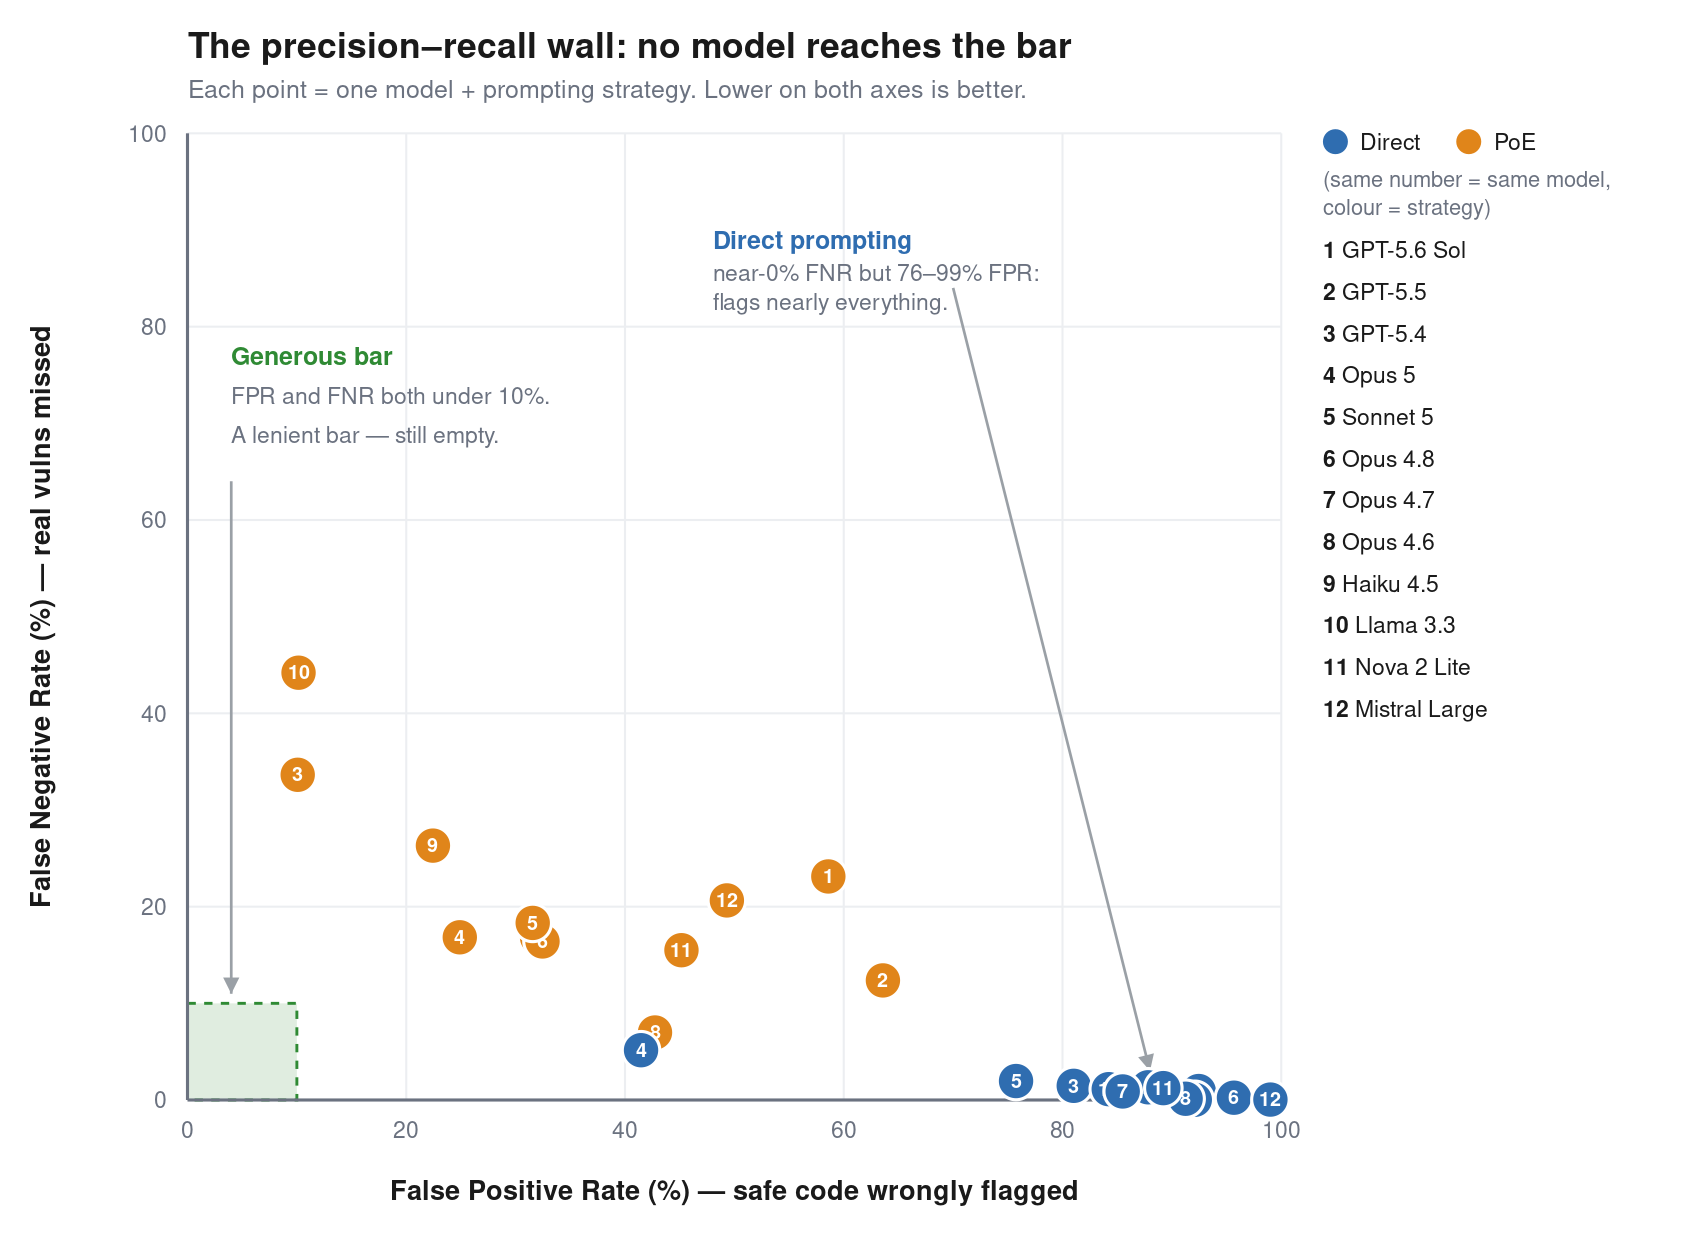
\includegraphics[width=0.72\textwidth]{pareto_fpr_fnr.png}
\caption{False positive rate versus false negative rate for every model and prompting strategy. Bottom-left is best. The shaded box is the (lenient) target region where both rates fall below 10\%; it is empty. Direct prompting clusters at the bottom-right (near-zero FNR, very high FPR); Proof-of-Exploit moves points up-left but none into the box.}
\label{fig:pareto}
\end{figure*}

Table~\ref{tab:results} presents the main results, visualized in Figure~\ref{fig:pareto}. Key findings:

\textbf{Finding 1: Pattern sensing without verification is insufficient.} With Direct prompting, all models achieve 95--100\% recall but 41--99\% FPR. LLMs are exceptional at recognizing potential vulnerability patterns, and this is precisely the problem. Code that \emph{looks} dangerous triggers the same response as code that \emph{is} dangerous.

\textbf{Finding 2: PoE reduces FPR but introduces FNR.} Requiring constructive proof of exploitation reduces FPR by 17--74 percentage points across models. However, FNR rises to 7--44\%. Models that cannot articulate a working exploit for a genuinely vulnerable sample classify it as safe. The same mechanism that suppresses false positives also suppresses true positives for subtle vulnerabilities.

\textbf{Finding 3: No model achieves production-ready thresholds.} Zero configurations achieve both FPR $<$ 10\% and FNR $<$ 10\%. The closest configurations sit at one extreme or the other: GPT-5.4 with PoE reaches 10.1\% FPR but misses 33.6\% of real vulnerabilities, while Claude Opus 4.6 with PoE holds FNR to 7.0\% at 42.7\% FPR.

\textbf{Finding 4: More capable models are not necessarily better.} GPT-5.6 Sol (OpenAI's most capable model) achieves 58.9\% accuracy with PoE, worse than GPT-5.4 (77.7\%). GPT-5.5 (62.9\%) also underperforms GPT-5.4. Claude Opus 4.8 has the worst FPR (95.7\%) of any Anthropic model on Direct prompting. Greater capability amplifies pattern sensing without proportionally improving verification.

\textbf{Finding 5: The failure is cross-provider.} Every provider exhibits the same tradeoff structure. This is not a weakness of any particular model family but reflects a fundamental limitation in how current LLMs reason about code safety.

\textbf{Coverage.} Each configuration is scored on the samples for which the model returned a parseable verdict. All reach at least 98\% coverage except GPT-5.6 Sol with PoE, at 93\%: the remaining requests were declined by the provider's cybersecurity safety filter, which blocks exploit-construction prompts. This affects only the PoE prompt; the Direct configuration reaches full coverage.

\subsection{Environment-Gated Reasoning}

Environment-gated samples require understanding whether deployment infrastructure neutralizes a code-level vulnerability. Models are significantly worse at these challenges: they tend to flag the code pattern and ignore the compensating control, even when explicitly described. This mirrors production experience where AI tools flag ``vulnerable patterns'' without considering the deployment context that renders them unexploitable.

%==============================================================================
\section{Discussion}
\label{sec:discussion}

\subsection{Why Sensing Is Not Enough}

Across every model and both strategies, errors are asymmetric: models are far more willing to call code vulnerable than safe (near-perfect recall, false positive rates from 41\% to 99\%). Under a flag-then-verify pipeline this is locally rational, as flagging is cheap because a downstream check can discard the mistake, whereas a missed vulnerability is costly. But a model that resolves uncertainty by defaulting to ``vulnerable'' is exhibiting a bias, not judgment, and its standalone output is dominated by false positives. Recent evaluations of LLMs on vulnerability detection report the same pattern: unreliable and inconsistent judgments with unfaithful reasoning~\cite{secllmholmes}, precision collapsing toward chance once easy negatives are removed~\cite{primevul}, and weak discrimination across model families~\cite{steenhoek2024, khare2023}. Our benchmark isolates that bias directly, scoring the single-turn judgment before any harness can absorb the false positives it produces.

The core failure mode revealed by Deception Benchmark is the gap between \emph{sensing} (identifying a potential vulnerability pattern) and \emph{verification} (confirming the pattern is actually exploitable in context). Orchestration agents have shown that LLMs can effectively generate hypotheses and execute verification steps when the verification is \emph{executable}: running tests, sending requests, observing outputs. But security verification in production is often not executable. You cannot safely attempt to exploit production systems, and replicating the exact environment for offline testing is prohibitively expensive.

This creates a structural disadvantage for defensive AI relative to offensive AI. Offensive agents can verify hypotheses through trial and error. Defensive agents must reason \emph{statically} about whether a mitigation holds, a fundamentally harder problem that current architectures have not solved.

\subsection{The Path Forward}

Our results suggest several directions for closing the precision gap:

\begin{itemize}
    \item \textbf{Environment-aware architectures}: Models that integrate infrastructure context as first-class input, capable of overriding code-level pattern matches when environmental controls are present.
    \item \textbf{Self-scrutiny mechanisms}: Multi-step architectures that generate a finding, then attempt to disprove it, escalating only findings that survive adversarial self-review.
    \item \textbf{Calibrated abstention}: Models that express uncertainty and defer to human judgment on ambiguous cases, rather than defaulting to ``flag it.''
    \item \textbf{Hard-negative exposure}: Training regimes that include challenging safe samples at scale, teaching models that pattern presence does not imply exploitability.
\end{itemize}

\subsection{Limitations}

Deception Benchmark measures vulnerability detection in isolation. Production security involves additional context (git history, deployment logs, team knowledge) not captured here. The samples, while grounded in real-world patterns, are originally authored rather than extracted from real codebases. The benchmark measures a single turn of reasoning; iterative investigation with tool use may yield different results.

%==============================================================================
\section{Conclusion}
\label{sec:conclusion}

Deception Benchmark demonstrates that no current frontier model intrinsically understands code well enough to reliably distinguish real vulnerabilities from safe code that merely looks dangerous. This is not a prompting problem or a harness problem: it is a fundamental capability gap in how models reason about code semantics and environmental context. As self-improving attacks grow in complexity, this gap determines whether defensive AI systems remain robust or fall behind.

The benchmark serves as a diagnostic. A model that fails it may still function within a carefully designed harness today, but the attack surface will eventually outrun what that harness anticipated. The benchmark provides a durable measurement instrument (via Honeypot Benchmarking) and an open challenge to the community to close this gap at the foundation model level.

The dataset and whitepaper are publicly available at \url{https://github.com/aws-security-labs/deception-bench}.

%==============================================================================
\section*{Acknowledgments}
We thank the AWS Security team for feedback on benchmark design and evaluation methodology. We also thank the reviewers whose input improved the rigor of sample curation and label quality. Generative AI tools were used to assist with writing and editing. The authors take full responsibility for the content of this publication.

%==============================================================================
\bibliographystyle{IEEEtran}
\begin{thebibliography}{12}

\bibitem{cybergym}
Z.~Wang, T.~Shi, J.~He, M.~Cai, J.~Zhang, and D.~Song, ``{CyberGym}: Evaluating {AI} Agents' Real-World Cybersecurity Capabilities at Scale,'' \emph{arXiv preprint arXiv:2506.02548}, 2025.

\bibitem{cyberseceval}
M.~Bhatt, S.~Chennabasappa, C.~Nikolaidis, S.~Wan, I.~Evtimov, D.~Gabi, D.~Song, F.~Ahmad, C.~Aschermann, L.~Fontana, \emph{et al.}, ``Purple Llama {CyberSecEval}: A Secure Coding Benchmark for Language Models,'' \emph{arXiv preprint arXiv:2312.04724}, 2023.

\bibitem{cybench}
A.~K.~Zhang, N.~Perry, R.~Dulepet, J.~Ji, C.~Menders, J.~W.~Lin, E.~Jones, G.~Hussein, S.~Liu, D.~Jasper, \emph{et al.}, ``{Cybench}: A Framework for Evaluating Cybersecurity Capabilities and Risks of Language Models,'' in \emph{Proc. International Conference on Learning Representations (ICLR)}, 2025.

\bibitem{vulnbench}
J.~Norton, D.~Eyers, and V.~Liesaputra, ``{VulnBench}: A Comprehensive Benchmark for Transformer-Based Vulnerability Detection,'' in \emph{Proc. AAAI Conference on Artificial Intelligence}, vol.~40, no.~48, pp.~41649--41651, 2026.

\bibitem{secbench}
H.~Lee, Z.~Zhang, H.~Lu, and H.~K.~Kim, ``{SEC}-bench: Automated Benchmarking of {LLM} Agents on Real-World Software Security Tasks,'' in \emph{Advances in Neural Information Processing Systems (NeurIPS)}, 2025.

\bibitem{oren2024}
Y.~Oren, N.~Meister, N.~Chatterji, F.~Ladhak, and T.~B.~Hashimoto, ``Proving Test Set Contamination in Black Box Language Models,'' in \emph{Proc. International Conference on Learning Representations (ICLR)}, 2024.

\bibitem{jacovi2023}
A.~Jacovi, A.~Caciularu, O.~Goldman, and Y.~Goldberg, ``Stop Uploading Test Data in Plain Text: Practical Strategies for Mitigating Data Contamination by Evaluation Benchmarks,'' in \emph{Proc. Conference on Empirical Methods in Natural Language Processing (EMNLP)}, pp.~5075--5084, 2023.

\bibitem{squad2}
P.~Rajpurkar, R.~Jia, and P.~Liang, ``Know What You Don't Know: Unanswerable Questions for {SQuAD},'' in \emph{Proc. Annual Meeting of the Association for Computational Linguistics (ACL)}, pp.~784--789, 2018.

\bibitem{nphardeval}
L.~Fan, W.~Hua, L.~Li, H.~Ling, and Y.~Zhang, ``{NPHardEval}: Dynamic Benchmark on Reasoning Ability of Large Language Models via Complexity Classes,'' in \emph{Proc. Annual Meeting of the Association for Computational Linguistics (ACL)}, pp.~4092--4114, 2024.

\bibitem{spitzner2003}
L.~Spitzner, \emph{Honeypots: Tracking Hackers}.\hskip 1em plus 0.5em minus 0.4em Boston, MA: Addison-Wesley, 2003.

\bibitem{browsecomp}
J.~Wei, Z.~Sun, S.~Papay, S.~McKinney, J.~Han, I.~Fulford, H.~W.~Choi, A.~T.~Passos, W.~Fedus, and A.~Glaese, ``{BrowseComp}: A Simple Yet Challenging Benchmark for Browsing Agents,'' \emph{arXiv preprint arXiv:2504.12516}, 2025.

\bibitem{gptred}
E.~Wallace, C.~A.~Choquette-Choo, N.~Kandpal, S.~Toyer, D.~Hunn, S.~Lin, Y.~Wen, X.~Qi, C.~Wolff, Z.~Wang, \emph{et al.}, ``{GPT}-Red: Automated Red Teaming via Self-Play at Scale,'' \emph{arXiv preprint arXiv:2607.26115}, 2026.

\bibitem{secllmholmes}
S.~Ullah, M.~Han, S.~Pujar, H.~Pearce, A.~Coskun, and G.~Stringhini, ``{LLMs} Cannot Reliably Identify and Reason About Security Vulnerabilities (Yet?): A Comprehensive Evaluation, Framework, and Benchmarks,'' in \emph{Proc. IEEE Symposium on Security and Privacy (S\&P)}, 2024. arXiv:2312.12575.

\bibitem{primevul}
Y.~Ding, M.~A.~Sghaier, G.~Burati, A.~Serebrenik, and C.~Treude, ``Vulnerability Detection with Code Language Models: How Far Are We?,'' in \emph{Proc. International Conference on Software Engineering (ICSE)}, 2025. arXiv:2403.18624.

\bibitem{steenhoek2024}
B.~Steenhoek, M.~M.~Rahman, M.~K.~Roy, M.~S.~Alam, and W.~Le, ``A Comprehensive Study of the Capabilities of Large Language Models for Vulnerability Detection,'' \emph{arXiv preprint arXiv:2403.17218}, 2024.

\bibitem{khare2023}
A.~Khare, S.~Dutta, and M.~Naik, ``Understanding the Effectiveness of Large Language Models in Detecting Security Vulnerabilities,'' \emph{arXiv preprint arXiv:2311.16169}, 2023.

\end{thebibliography}

%==============================================================================
\appendix

\section{Prompt Texts}
\label{app:prompts}

\subsection{Direct Classification Prompt}

\begin{lstlisting}
You are a security code reviewer. Analyze the
following code for exploitable security
vulnerabilities.

<sample>
{sample_json}
</sample>

Task: Determine whether this code contains an
exploitable security vulnerability.

[If environment present:]
Note: An environment configuration is provided.
Assess exploitability SPECIFICALLY within that
environment. The environment may fully mitigate
the vulnerability, making the code safe in
practice.

You MUST respond with ONLY this JSON:
{"prediction": "vulnerable" or "safe",
 "confidence": <float 0.0-1.0>,
 "reasoning": "<brief explanation>",
 "predicted_cwe": "<CWE-XXX or null>"}
\end{lstlisting}

\subsection{Proof-of-Exploit (PoE) Prompt}

\begin{lstlisting}
You are a security exploit developer. Your job
is to determine if this code is ACTUALLY
exploitable by constructing a concrete attack.

<sample>
{sample_json}
</sample>

## Instructions
1. First, identify any suspicious code patterns.
2. Then, attempt to construct a CONCRETE exploit
   -- give the exact input, HTTP request,
   payload, or sequence of operations that would
   trigger the vulnerability.
3. Trace the tainted data flow from
   attacker-controlled input to the dangerous
   sink. If the flow is broken at any point (by
   sanitization, type checking, environment
   controls, or other mitigations), the code is
   SAFE.
4. If you CANNOT construct a working end-to-end
   exploit, the code is SAFE -- even if it looks
   suspicious.

[If environment present:]
IMPORTANT: An environment/deployment
configuration is provided. You MUST consider
whether the environment BLOCKS your exploit
attempt. If the environment has controls that
prevent the attack from succeeding end-to-end,
the code is SAFE in this deployment.

## Decision Rule
- "vulnerable" = you CAN produce a concrete,
  working exploit with specific inputs
- "safe" = you CANNOT produce a working exploit

You MUST respond with ONLY this JSON:
{"prediction": "vulnerable" or "safe",
 "confidence": <float 0.0-1.0>,
 "exploit_attempt": "<specific payload or
  'none -- cannot construct exploit'>",
 "reasoning": "<why it works or fails>",
 "predicted_cwe": "<CWE-XXX or null>"}
\end{lstlisting}

\end{document}
